% load FRI thesis document class with options: 
% - language=english for writing in english as main language [default]
% - language=slovene for writing in slovene as main language
% - funding=logo.pdf for a funded PhD thesis - doktorska disertacija MR iz gospodarstva, 
% - stage=pre-alpha for early drafts - no chapter thumbs, smaller page size, which leads to increased font sizes when printed on A4 fit to page [seeks for images in directories /img_LQ, /img]
% - stage=alpha for first review by advisor - no chapter thumbs, smaller page size, which leads to increased font sizes when printed on A4 fit to page [seeks for images in directories /img_LQ, /img]
% - stage=beta for seminar 5 - no chapter thumbs, smaller page size, which leads to increased font sizes when printed on A4 fit to page [seeks for images in directories /img_LQ, /img]
% - stage=gamma for senate aproval - no chapter thumbs, TODO: includes notes showing reviewer comments (and author response) [seeks for images in directories /img_LQ, /img]
% - stage=gold for final approved version - notes not displayed, chapter pages in colour, chapter thumbs [seeks for images in directories /img_LQ, /img]
% - stage=press for print version - gold with trimmarks [seeks for images in directories /img_HQ, /img]
\documentclass[language=english,stage=gold]{FRIteza}

\author[A={D Author}]{Demo Author}

\title[language=english]{Demo thesis title}
\title[language=slovene]{Naslov demo disertacije}

\keywords[language=english]{template, demo, doctoral, thesis}
\keywords[language=slovene]{predloga, demo, doktorska, disertacija}

% primer v slovenskem jeziku
%\approvedBy[title={profesor za računalništvo in informatiko}, role={mentor}]{dr. Main Mentor}
%\approvedBy[title={profesor za računalništvo in informatiko}, role={predsednik ocenjevalne komisije}]{dr. Examiner Chair}
%\approvedBy[title={izredni profesor za računalništvo in informatiko}, role={predsednik ocenjevalne komisije}]{dr. Examiner Two}
%\approvedBy[affiliation={University of Abroad}, title={Professor Emeritus of Thesis Topic}, role={zunanji član ocenjevalne komisije}]{dr. Examiner Three}
\approvedBy[title={Professor of Computer and Information Science}, role={advisor}]{dr. Main Mentor}
\approvedBy[title={Professor of Computer and Information Science}, role={examiner}]{dr. Examiner Chair}
\approvedBy[title={Associate Professor of Computer and Information Science}, role={examiner}]{dr. Examiner Two}
\approvedBy[affiliation={University of Abroad}, title={Professor Emeritus of Thesis Topic}, role={external examiner}]{dr. Examiner Three}

\previousPublication{%
	Author D, Mentor M (2003) 
	Main thesis results manuscript, in
	\emph{High-impact conference}, 
	Lecture Notes in Doctoral Topic, Vol. 13,
	eds. Editor O, Editor T
	(Demo Publisher, Berlin), 
	doi:\,\doi{10.nnnn/n-nnn-nnnnn}.
}
\previousPublication{%
	Author D (15/04/2005)
	\emph{Main topic of doctoral disertation}. 
	Invited lecture, University of Abroad, Department of Research, City.
}
\previousPublication{%
	Author D, Mentor M (2005) 
	Main thesis results manuscript.
	\emph{Journal of High-Impact}
	doi:\,\doi{10.nnnnn/n.nnnn.nnnn.nn.nnn}.
}

% force correct date display, ignored if stage not gold or press
\forceDate{1}{2019}

% define cover 
% \cover[title=<title to appear on cover page>, loc=<location of the title>, colour=<colour of the title>]{coverImage}
% defaults: title=\title{#}, loc=NE, colour=P1797
% notes:
%  title - use title to insert prefered line breaking with '\\' 
%  loc - options NE, SE, NW, SW
%  colour - options P1797, white, black
%\cover[title={Fuzzy model for a computer simulation of bird flocking}, loc={NE}, colour={P1797}]{./cc/coverImage.jpg} 
% define spine
% \spine[title=<title to appear on spine>, loc=<location of the title>, colour=<colour of the title>]{thesisId in hexadecimal}
% defaults: title=\title[A={#}]
% notes:
%  title - use title to provide a shortended title for the spine 
%  pages - privde the total number of pages
%\spine[title={Fuzzy model for a computer simulation of bird flocking}, pages=134]{80}

% load path for graphics files
%\graphicspath{{img/}}
%\DeclareGraphicsExtensions{.pdf,.png,.jpg} % search order for graphics files

\usepackage{xspace} % helper package for automatic spaces after replacement macros, to be used with caution
%% define common abbreviations
\newcommand{\ie}{i.e.\xspace} % id est ~ that is
\newcommand{\eg}{e.g.\xspace} % exempli gratia ~ for example
\newcommand{\etc}{etc.\xspace} % et cetera ~ and so on
\newcommand{\etal}{\xspace et al.\xspace} % et al. ~ and others
\newcommand{\fig}{Fig.} % reference a figure
\newcommand{\figs}{Figs.} % reference multiple figures
\newcommand{\tab}{Tab.} % reference a table

%% define macros for frequently used commands 
\newcommand{\eng}[1]{angl. #1} % english original

%% notation
\newcommand{\R}{\Rset} \newcommand{\Rset}{\ensuremath{\mathbb{R}}} % real numbers symbol
\newcommand{\N}{\Nset} \newcommand{\Nset}{\ensuremath{\mathbb{N}}} % natural numbers symbol
\newcommand{\E}{\Eset} \newcommand{\Eset}{\ensuremath{\mathbb{E}}} % euclidean vector space symbol
\newcommand{\set}[1]{{\ensuremath{\symbfup{#1}}}} % set; introduction + 
\newcommand{\powset}[1]{\ensuremath{\mathcal{P}(#1)}} % power set; introduction +  
\newcommand{\vect}[1]{\ensuremath{\symbfup{#1}}} % vector; introduction + 
\newcommand{\autom}[1]{{\ensuremath{\symrm{#1}}}} % automaton; animat
%
\newcommand{\fset}[1]{{\ensuremath{\tilde{\set{#1}}}}} % fuzzy set; introduction +  
\newcommand{\fpowset}[1]{\ensuremath{\symcal{F}(#1)}} % fuzzy power set; introduction +  
\newcommand{\fautom}[1]{\ensuremath\tilde{\symup{#1}}} % fuzzy automaton; fuzzyanimat
\newcommand{\ffunc}[1]{\ensuremath\tilde{#1}} % fuzzy function; fuzzyanimat
%
\newcommand{\fvar}[1]{\emph{#1}} % fuzzy variable; fuzzymodelling
\newcommand{\kwd}[1]{\textsc{#1}} % keyword; fuzzymodelling
\newcommand{\fval}[1]{\emph{#1}} % fuzzy value; fuzzymodelling
\newcommand{\frule}[1]{\textsc{\MakeLowercase{#1}}} % fuzzy rule; fuzzymodelling
\newcommand{\statement}[1]{\ensuremath\mathscr{#1}} % logical statement; fuzzymodelling
%
\DeclareMathOperator*{\sgn}{sgn} % sign operator; fuzzyanimat
\DeclareMathOperator*{\cog}{cog} % centre of gravity operator; fuzzymodelling
%
\newcommand{\aprod}{\ensuremath\capdot} % algebraic product symbol
%
\newcommand{\fov}{\ensuremath\mathit{fov}} % field of view; \mathit ensures proper kerning between f and o, a common issue for multichar variables

% define additional hyphenation patterns
\sethyphenation{english}{pri-mar-i-ly} % https://www.hyphenation24.com/


\usepackage{lipsum}
\usepackage{blindtext}

\begin{document}

% TODO: show as an example of subfigure use
%\begin{figure}
%	\begin{subfigure}[b]{.5\figurewidth-3.5pt}
%		\noindent\hrulefill\par
%		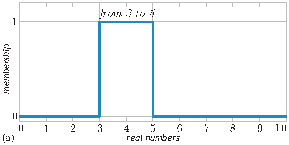
\includegraphics{fig_fuzzySet_a}
%		\caption{sub A}\label{labA}
%	\end{subfigure}
%	\hfill
%	\begin{subfigure}[b]{.5\figurewidth-3.5pt}
%		\noindent\hrulefill\par
%		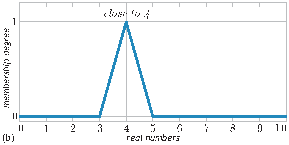
\includegraphics{fig_fuzzySet_b}
%		\caption{sub B}\label{labB}
%	\end{subfigure}
%	\caption{Membership functions of a crisp set of real numbers `from 3 to 5' \subref{labA} and a fuzzy set of real numbers `close to 4' \subref{labB}.}
%	\label{fig:fuzzy:set0}
%\end{figure}

\frontmatter
	\maketitle
	\makeapprovedby
	\makepreviouspublication
	% !TeX root = ./thesis.tex










%==============================
\cleardoublepage
\thispagestyle{empty}

\vspace*{55pt}

\begin{centering}

{\textsc{in memoriam}
 \par}

\vspace{.5cm}

{Damjan Oseli
 \par}

{1975--2004
 \par}

\end{centering}

\vfill






%==============================
\cleardoublepage
\thispagestyle{empty}

\vspace*{55pt}

\begin{centering}

{\setbox0=\hbox{\emph{``Things never turn out the way you think they will.''}}
 \begin{minipage}{\wd0}
 \emph{``Things never turn out the way you think they will.''}\\
 \null \hfill  --- Michael Crichton, \emph{Prey}, 2002.
 \end{minipage}
 \par}

\vspace{.5cm}

{\setbox0=\hbox{
\includegraphics{pixar_forTheBirds}}
 \begin{minipage}{\wd0}
 
\includegraphics{pixar_forTheBirds}\\
 \null \hfill  --- Pixar, \emph{For the Birds}, 2000.
 \end{minipage}
 \par}

\end{centering}

\vfill
\cleardoublepage

	% !TeX root = ./thesis.tex

% write thesis abstracts
% use \begin{abstract}\end{abstract} for abstract in english
% use \begin{povzetek}\end{povzetek} for abstract in slovene
% note
% with english as primary language the order is povzetek, abstract
% with slovene as primary language the order is abstract, povzetek


%==============================
\begin{povzetek}

%-----
\lipsum[2-4]

\end{povzetek}


%==============================
\begin{abstract}

%-----
\lipsum[2-4]

\end{abstract}

	% !TeX root = ./thesis.tex

% Do thank those that have helped you








%==============================
\begin{acknowledgements}

Along my epic journey as a PhD student I was lucky enough to have met and shared parts of this pilgrimage with a number of interesting characters. Not to leave anyone out or have the acknowledgements take the major part of this book, I will, from now on, write as if we all contributed to this work (in fact we did, one way or another).

\end{acknowledgements}

\vfill

\begin{center}
	\textsc{This thesis was partially funded by the European Social Fund.}
	
	\vspace{.2cm}
	
	\textsc{Credits for the stuning photo on the cover go to Ed Ralph.}
\end{center}
	\tableofcontents 

\mainmatter
	% !TeX root = ./thesis.tex










%==============================
\chapter{Introduction}
\label{ch:introduction}


%-----
\section{Motivation}
With the increase of the processing and presentational capabilities of personal computers, the field of computer modelling and simulation has been gaining research interest even in the areas that a decade ago did not believe that modelling and simulation were suitable for them. One such area is the modelling of the dynamics of organized groups of moving animals. Some of the typical examples of such groups are pedestrians \cite{brogan:1998,helbing:1995}, bird flocks and fish schools \cite{aoki:1982,heppner:1990,lebar_bajec:2002,lebar_bajec:2003a,lebar_bajec:2003b,lebar_bajec:2005a,okubo:1986,reynolds:1987,terzopoulos:1994,tu:1994,tu:1999,zaera:1996}, ant colonies \cite{bonabeau:1999,resnick:1997}, \etc\ For the majority of these groups their dynamics is not based on a centralized source of decision processing, but on a distributed one. Each individual member of the group thus processes its own decision, depending on the perceived state of the universe and the tendencies that originate from the drives guiding it.

If I focus on bird flocks: the first and most influential models were developed by Reynolds \cite{reynolds:1987} and Heppner and Grenander \cite{heppner:1990}. In both cases the drives are implemented through mathematical equations (geometrical calculations, differential equations, \etc), which the authors obtained by means of trial-and-error experimentation. According to Reynolds \cite{reynolds:1987,reynolds:1999}, these drives are:

\begin{itemize}
  \item \emph{separation}: each member of the flock tries to maintain a certain separation distance from its flockmates (nearby flock members),

  \item \emph{alignment}: each member of the flock tries to match its flight speed and flight direction with that of its flockmates,

  \item \emph{cohesion}: each member of the flock tries to fly toward the centre of its flockmates.
\end{itemize}

According to Heppner and Grenander \cite{heppner:1990}, the drives are:

\begin{itemize}
  \item \emph{homing}: each member of the flock tries to stay in the roosting area,

  \item \emph{velocity regulation}: each member of the flock tries to fly with a certain predefined flight speed---it tries to return to that speed if perturbed,

  \item \emph{interaction}: if two flockmates are too close to one another, they try to move apart; if they are too distant, they do not influence each other; otherwise they try to move closer together.
\end{itemize}

However, in addition to these three drives, Heppner and Grenander modelled also the \emph{random impact}, which was intended to simulate the random distractions that are present in a natural environment (wind gusts, distractions from moving objects on the ground, \etc). They implemented it as a Poisson stochastic process and admitted that without its inclusion they were unable to produce flock-like behaviour.

Upon the analysis of the relevant bibliography it has been determined that the existing models have some weaknesses, which can be briefly summarized as follows:

\begin{itemize}
  \item \emph{syntactical confusion}: most of the authors do not present formal definitions of the models; in the majority of cases the models are only described, which is usually not a good enough basis for an actual implementation; the latter requires a formal specification in the form of an automaton or algorithm;

  \item \emph{lack of evaluation metrics}: regardless of the numerous models, neither an analytical comparison between the obtained results nor their evaluation have been performed; in this sense the models have never been truth-tested;

  \item \emph{usability}: most of the models are based on complex mathematical formalisms (differential equations, random processes, computation of the centre of mass, \etc); in this sense the models are difficult to understand and/or use by the audience they were designed for (biologists, ethologists, behaviourists, etc.).
\end{itemize}

Fuzzy modelling has gained momentum with the increase of processing capabilities. It is based on fuzzy logic, which emerged as an outgrowth of fuzzy set theory. The latter was first introduced in 1965 by Lotfi A. Zadeh \cite{zadeh:1965}. Fuzzy set theory is a generalization of conventional (or crisp) set theory by the introduction of the concept of partial membership. The main difference between the two is thus in the interpretation of membership. In conventional set theory, an object can be either a member of the observed set or not a member of the observed set; in fuzzy set theory, however, it can also be a partial member of the observed set. Therefore if the object's membership to the observed set is computed by means of a membership function, then in the case of a crisp set this function maps to the set $\left\{0,1\right\}$, whereas in the case of a fuzzy set it maps to the entire unit interval $\left[0,1\right]$.

The basics of modelling using uncertain knowledge and preconditions were set by Witold Pedrycz \cite{pedrycz:1993}. In the current literature numerous examples of fuzzy modelling can be found (modelling of fire spread prediction \cite{mraz:1999,vakalis:2004a,vakalis:2004b}, modelling of snow avalanches \cite{barpi:2004}, modelling of the control of kitchen appliances \cite{mraz:2001}, \etc). However, only some of them model massive dynamic processes. Furthermore in the extensive literature I did not find any attempt at fuzzy modelling of bird flocking.


%----
\section{Scientific Contributions}
In the light of the preceding discussion about the existing models' weaknesses, the following scientific contributions are presented in this dissertation:

\begin{itemize}
  \item \emph{design and formal definition of an extended Moore automaton (animat)}:
  with respect to the current syntactical confusion I design and present a formal definition of an extended Moore automaton \cite{kohavi:1978}, which allows a uniform approach to modelling the dynamics of organized groups of moving entities; the ideas behind the above mentioned formal definition correspond with the term animat, which was introduced, without a formal definition, by Wilson \cite{wilson:1985}; in spite of that, in the last decade the term has become the synonym for a class of computer simulated animals or robots;

  \item \emph{design and formal definition of a fuzzy extended Moore automaton (fuzzy animat)}:
  afterwards I upgrade the extended Moore automaton with the introduction of fuzziness \cite{zadeh:1965}; the latter allows the construction and implementation of the automaton by using ambiguous (uncertain, vague, \etc) knowledge and data; one of the main advantages of fuzzy logic is its ability to permit a direct linguistic description (programming) of an arbitrary decision system;

  \item \emph{application of the fuzzy animat to the problem of the simulation of bird flocking}:
  to present its usability I employ the fuzzy animat to model a member of a bird flock; the model is limited to a two-dimensional space without obstacles; these two preconditions originate from comparable models of other authors;

  \item \emph{design and formal definition of a set of metrics used for comparing the simulation results from different computer models of bird flocking}:
  the authors of the related models base the analysis of their simulation results mostly on visual grounds; the approach is subjective and is, as such, useless for an analytical comparison of different models; with this in mind I design and formally define a set of metrics that allow the comparison of the simulation results, and if the required data be available, perhaps also a comparison to the dynamics of a natural flock;

  \item \emph{comparison of the simulation results obtained by using different computer models of bird flocking}:
  I then use the introduced metrics to compare the simulation results obtained by using the newly introduced model with those obtained by using Reynolds's model \cite{reynolds:1987,reynolds:1999}; the latter represents the main reference for the majority of the existing models;

  \item \emph{analysis of simulation results from different computer models of bird flocking}:
  I analyse the differences in the simulation results of the compared models.
\end{itemize}


%----
\section{Methodology}
In the quest to achieve the discussed scientific contributions, the following methodologies have been employed:

\begin{itemize}
\item review and analysis of the bibliography related to modelling massive dynamic processes; in doing so, I have learnt about the most important related models;
\item application of the acquired knowledge to the design of an extended Moore automaton (animat);
\item application of the knowledge about fuzzy logic to the design of a fuzzy extended Moore automaton (fuzzy animat);
\item development of a computer application (simulator) for the simulation of bird flocking;
\item experimental work with the simulator and analysis of the simulation results;
\item comparison of the results obtained with the simulation and those obtained by using the computer models of other authors;
\item monitoring and review of all of the new activities in the related fields and active participation in the form of journal articles and conference contributions.
\end{itemize}


%----
\section{Dissertation Overview}
The main question to be addressed by this dissertation is, ``How to use fuzzy logic for modelling bird flocking?'' I feel that flock-like behaviour could be much more easily described by using simple linguistic descriptions (\eg\ collections of if-then rules) than by using mathematical equations. Indeed, the existing knowledge about the behaviour of flocks is usually available in the form of the observer's linguistic descriptions and explanations of the perceived behaviour.\footnote{``\emph{It seems likely that if a bird, say, to the left and in front of another bird turned suddenly in front of the trailing bird, the trailing bird would have time to react, and turn in the same direction, avoiding collision.}'' From personal correspondence with Frank H. Heppner.} The existing models were thus arrived at by approximating such linguistic descriptions using mathematical equations. Moreover, considerable amounts of advanced mathematical skills were required for this transition. Fuzzy logic \cite{zadeh:1965} is a very popular, successful and widespread approach for modelling processes, for example fire spread prediction \cite{mraz:1999,vakalis:2004a,vakalis:2004b}, which are too complex for classical mathematical methods. I feel that by using it to describe the simulated animal's behaviour the transition from the linguistic description to the actual behaviour could be made much shorter and much more understandable. In this way researchers involved with the study of the dynamics of organized groups of moving animals would gain a tool that enabled them to construct the subjects of their interest---the digital animals---and study their behaviour through simulations.

This dissertation presents the \emph{fuzzy animat construction framework} and through the study case of bird flocking also its usage. In \chaptername~\ref{ch:birdFlocks} the bird flocking literature is reviewed and the two most influential models are presented. \chaptername~\ref{ch:animat} presents a formal definition of an extended Moore automaton that can be used as a uniform approach to modelling the dynamics of organized groups of moving animals. \chaptername~\ref{ch:fuzzyModelling} presents a brief overview of fuzzy logic and fuzzy modelling. In \chaptername~\ref{ch:fuzzyAnimat} fuzzy logic is used to introduce fuzziness into the earlier formalized extended Moore automaton, which is then used to construct a fuzzy digital bird. \chaptername~\ref{ch:analysis} is dedicated to the analysis of the dynamics of organized groups of moving fuzzy digital birds and \chaptername~\ref{ch:conclusion} concludes by reviewing the achieved scientific contributions and presenting the future research directions.

I assume that the reader is familiar with the fundamentals of the theory of conventional (or crisp) sets and conventional (crisp or two-valued) logic. Furthermore, it is assumed that the reader is familiar with Euclidean vector spaces and corresponding vector operations. Throughout the dissertation I use the following notation:

\begin{itemize}
  \item $\N=\left\{1,2,3,\ldots\right\}$ the set of all positive natural numbers,
  \item $\N_n=\left\{1,2,3,\ldots,n\right\}$ the set of all positive natural numbers lower or equal $n$,
  \item $\R$ the set of all real numbers,
  \item $\R^+$ the set of all non-negative real numbers,
  \item $\E$ an Euclidean vector space such as $\R^2$, $\R^3$,
  \item $\set{A},\ldots,\set{Z}$ conventional (or crisp) sets,
  \item $\fset{A},\ldots,\fset{Z}$ fuzzy sets,
  \item $\vect{a},\ldots,\vect{z}$ vectors from vector space $\E$,
  \item $\langle x_1,x_2,\ldots,x_n \rangle$ ordered $n$-tuple of elements $x_1$, $x_2$, \ldots, $x_n$.
\end{itemize}

\noindent In addition
\begin{itemize}
  \item $\mathrm{iff}$ is shorthand expression for ``if and only if'',
  \item $\exists$ is shorthand expression for ``exists'',
  \item $\forall$ is shorthand expression for ``for all'',
  \item $\left|\set{A}\right|$ is shorthand for the size of set $\set{A}$,
  \item $\mu_\set{A}$ is shorthand for the membership function of crisp set $\set{A}$,
  \item $\powset{\set{A}}$ is shorthand for the family of all crisp sets that can be defined on universal set $\set{A}$,
  \item $\mu_\fset{A}$ is shorthand for the membership function of fuzzy set $\fset{A}$,
  \item $\fpowset{\set{A}}$ is shorthand for the family of all fuzzy sets that can be defined on universal set $\set{A}$,
  \item $\left\|\vect{a}\right\|$ is shorthand for the size (norm) of vector $\vect{a}$,
  \item $\vect{a}^0$ is shorthand for the normalized vector $\vect{a}$ (\ie\ a vector in the same direction as $\vect{a}$ but with size $1$),
  \item $\lfloor\vect{a}\rceil^a$ is shorthand for the truncated vector $\vect{a}$ (\ie\ a vector in the same direction as $\vect{a}$ but with size lower or equal $a$).
\end{itemize}

	% !TeX root = ./thesis.tex


%==============================
\chapter{Demo Chapter A}
\label{ch:ch2}


%-----
\section{Demo Section AA}
\label{sec:ds2A}
The most important related work was published in~\cite{demorefA:2000, demorefB:2001,demorefC:2002,demorefP:2003,demorefM:2004,demorefD:2005}

\blindtext


%-----
\section{Demo Section AB}
\label{sec:ds2B}
\blindtext

\subsection{Demo Subsection AB.1}
\label{sub:dss2B1}
\blindmathpaper

\subsubsection{Demo Subsubsection AB.1.1}
\label{sub:dss2B11}
\blindtext

\subsubsection{Demo Subsubsection AB.1.2}
\label{sub:dss2B12}
\blindtext

\subsection{Demo Subsection AB.2}
\label{sub:dss2B2}
\blindmathpaper


%-----
\section{Demo Section AC}
\label{sec:ds2C}
\blindmathpaper

	% !TeX root = ./thesis.tex


%==============================
\chapter{Demo Chapter B}
\label{ch:ch3}
\lipsum[30-31]

%-----
\section{Demo Section B1}
\lipsum[32-33]


%-----
\section{Demo Section B2}
\lipsum[34-35]


%-----
\section{Demo Section B3}
\lipsum[36-37]

	% !TeX root = ./thesis.tex


%==============================
\chapter{Demo Chapter C}
\label{ch:ch4}
\lipsum[40-41]


%-----
\section{Demo Section C1}
\lipsum[42-42]


%-----
\section{Demo Section C2}
\lipsum[44-45]


%-----
\section{Demo Section C3}
\lipsum[46-47]

	% !TeX root = ./thesis.tex


%==============================
\chapter{Demo Chapter D}
\label{ch:ch5}
\lipsum[50-51]


%-----
\section{Demo Section D1}
\lipsum[52-53]


%-----
\section{Demo Section D2}
\lipsum[54-55]

	% !TeX root = ./thesis.tex


%==============================
\chapter{Conclusion}
\label{ch:conclusion}
\lipsum[60-61]


%----
\section{Principal Scientific Contributions}
\lipsum[62-63]


%----
\section{Future Research Directions}
\lipsum[64-65]

	\begin{appendices}
	\end{appendices}

\backmatter
	% !TeX root = ./thesis.tex

% use bibtex for bibliography








%==============================
\bibliography{jd}

	% !TeX root = ./thesis.tex










%==============================
\begin{razsirjeniPovzetek}

%-----
\EBlettrine{Ali} imajo jate ptic, jate rib, črede kopitarjev, roji mušic, mehiški val, trume ljudi na koncertu, borza in biološke celice kaj skupnega? S tem se ukvarjajo znanstveniki, ki raziskujejo področje skupinskega vedenja. Primere skupinskega vedenja iz narave prikazuje slika~\ref{fig:CB_si}. Skupinsko vedenje je fascinantno področje, ki analizira, kako preproste odločitve posameznikov vplivajo na dinamiko celotne skupine. Aristotel je nekoč izjavil: »Celota je več kot vsota sestavnih delov.« -- trditev, ki zelo lepo opiše bistvo skupinskega vedenja. Rezultati raziskav iz področja skupinskega vedenja so zanimivi za znanstvenike z več različnih področij, od biologije, fizike in medicine do družboslovnih ved in računalništva \cite{deisboeck2009collective,lebarbajec2009organized,nahin2012chases,silverberg2013collective,spector2003emergence,sumpter2006principles,vicsek1995novel,wei2009pursuit,xu2014crowd}.

\begin{figure}[p]
	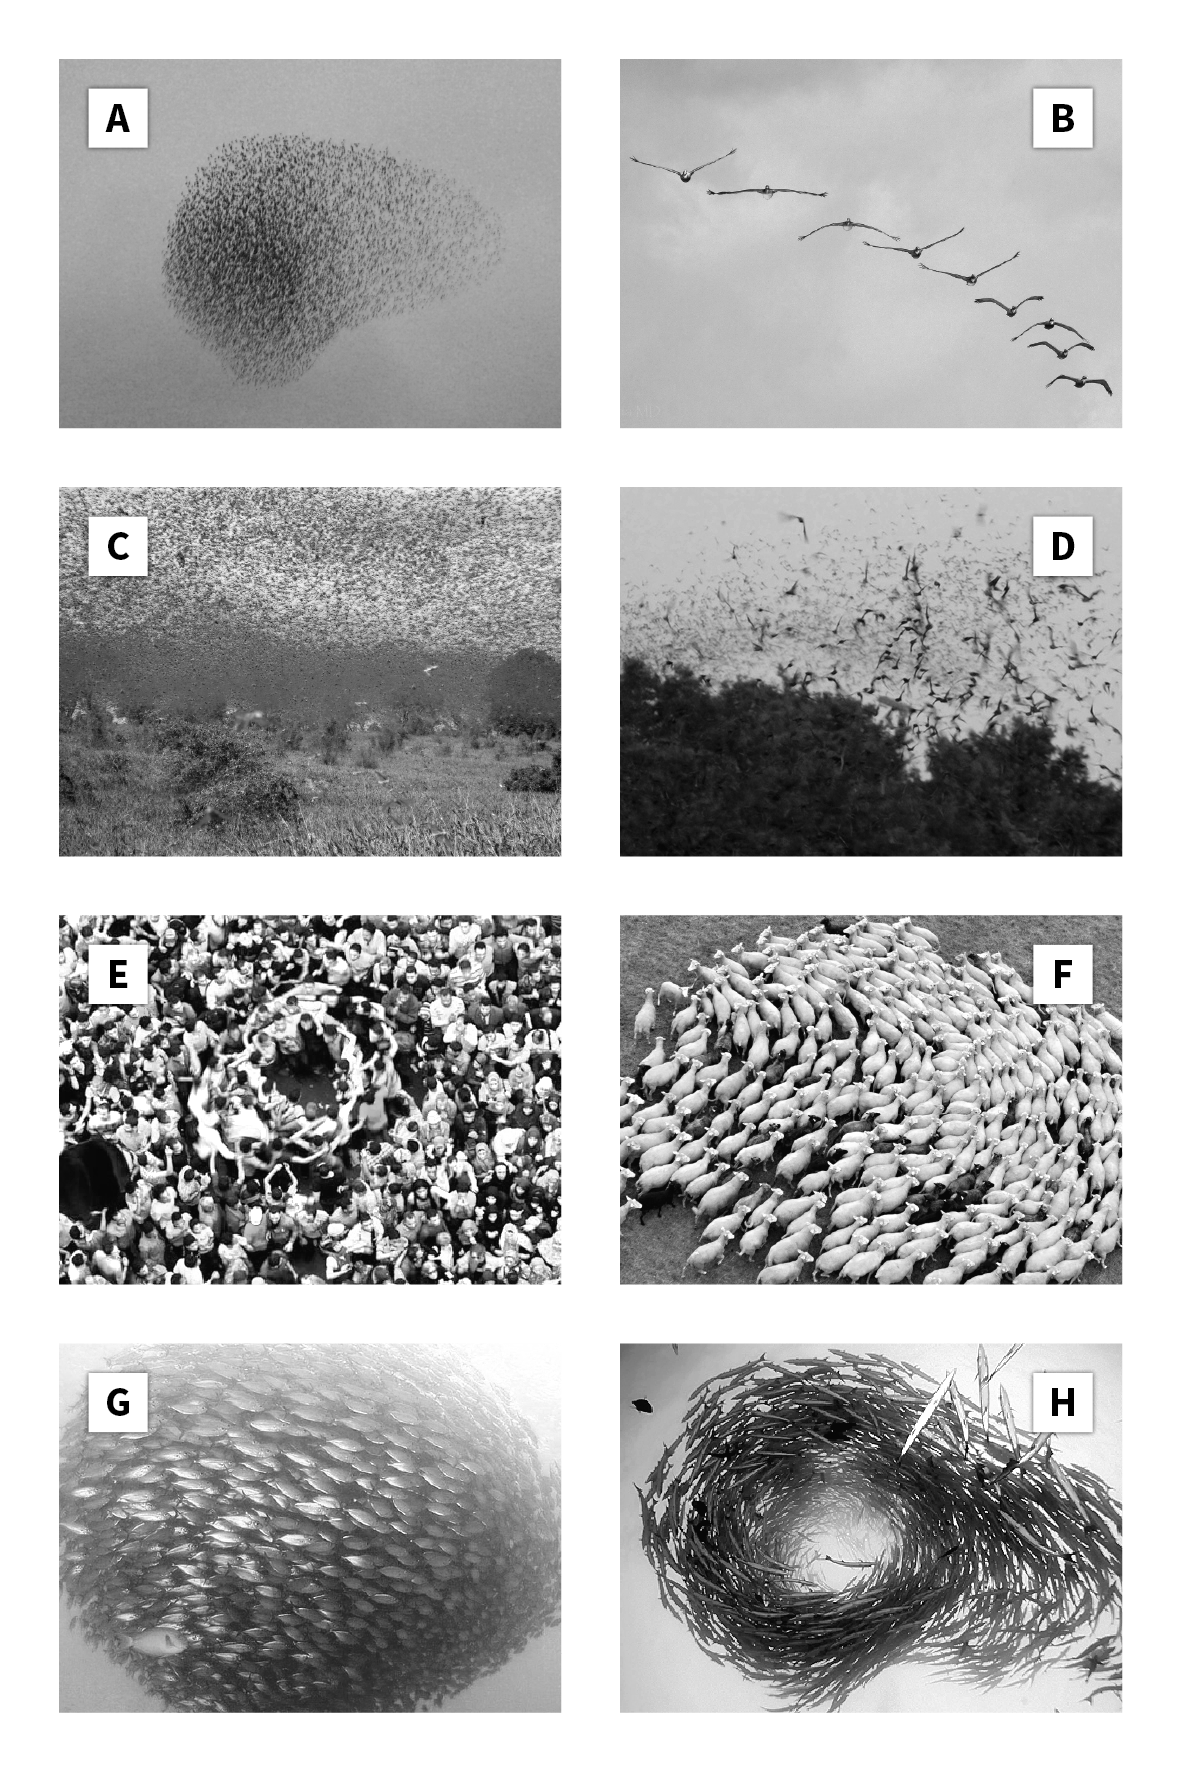
\includegraphics[width=\figurewidth]{figCB_BW.png}
	\caption{Primeri različnih režimov skupinskega vedenja, ki jih lahko opazimo v naravi. A) jata škorcev (© Tim Regan, \href{www.flickr.com}{flickr.com}). B) pelikani, ki letijo v formaciji (© Daniel D'Auria, \href{www.flickr.com}{flickr.com}). C) roj kobilic (© FAO emergencies, \href{www.flickr.com}{flickr.com}). D) roj netopirjev (© Amanda, \href{www.flickr.com}{flickr.com}). E) ljudje na koncertu (© Amanda Mustard, \href{http://www.amandamustard.com/}{amandamustard.com/}). F) čreda ovc (© Dariusz Paciorek, \href{http://www.aeroart.com.pl/}{aeroart.com.pl/}). G) ribe v jati, ki ima obliko krogle (© Bo Pardau, \href{www.flickr.com}{flickr.com}). H) kroženje rib okoli praznega jedra (© Robin Hughes, \href{www.flickr.com}{flickr.com}).}
	\label{fig:CB_si}
\end{figure}

Področje skupinskega vedenja (\angl{collective behaviour, collective animal behaviour, swarming behaviour}) je tako zelo aktualno, saj kljub temu, da gre za pojav, ki ga lahko praktično vsak dan srečamo v naravi, mnoga raziskovalna vprašanja ostajajo nerešena \cite{krause2002living,lebarbajec2009organized,sumpter2006principles}. Tako še vedno nismo povsem prepričani, zakaj se nekatere skupine živali (predvsem tiste, kjer se živali gibajo močno usklajeno) pravzaprav sploh tvorijo \cite{lebarbajec2009organized}. Zakaj v naravi obstaja toliko različnih oblik skupinskega vedenja? Zakaj zgolj nekaj vrst ptic, ki letijo v skupinah, to počne v močno usklajenih oblikah? Zakaj so si ptice, ki pripadajo sorodnim vrstam \cite{jarvis2014wholegenome}, po obliki skupinskega vedenja tako različne \cite{lebarbajec2009organized}? V literaturi o skupinskem vedenju lahko najdemo vrsto različnih, tudi nasprotujočih si hipotez o tem, zakaj se živali združujejo v skupine. Nekatere pravijo, da živali tako povečajo učinkovitost pri razmnoževanju in iskanju hrane \cite{krebs1994behavioural}, druge trdijo, da ribe in ptice z usklajenim gibanjem varčujejo z energijo \cite{hemelrijk2014increased,marras2015fish,portugal2014upwash}.

Verjetno najbolj pogosta hipoteza o skupinskem vedenju trdi, da pri živalih združevanje v skupine služi kot učinkovit obrambni mehanizem pred plenilci \cite{cresswell2011predicting,hart2005predator,krause2002living,larsson2012why,lebarbajec2009organized,nishimura2002predator,pavlov2000patterns}. Hipoteza o sebični čredi (\angl{the selfish-herd hypothesis}) trdi, da posamezne živali z združevanjem v skupine zmanjšujejo svoje območje ogroženosti \cite{hamilton1971geometry,viscido2001response}. Hipoteza o zmanjševanju tveganja (\angl{the dilution of risk hypothesis}) razlaga, da ima posameznik manjšo verjetnost, da bo izbran kot tarča plenilca v večjih skupinah \cite{tosh2011conditions}. Hipoteza mnogih oči (\angl{the many eyes hypothesis}) pravi, da se z velikostjo skupine zmanjšuje čas, ki ga mora za odkrivanje nevarnosti vsak posameznik nameniti opazovanju okolice \cite{elgar1989predator,haley2014exploring,ruxton2008application,sadedin1998influence} ter da se z večanjem skupine povečuje verjetnost pravočasne zaznave plenilca \cite{galton1871gregariousness}. Hipoteza o zmedljivosti (\angl{the confusability hypothesis}) predvideva, da ima plenilec težave pri izbiri in sledenju tarče, če se ta nahaja v skupini, ki si je medsebojno vizualno podobna \cite{demsar2015simulating,kunz2006prey,nishimura2002predator,olson2013predator,olson2016evolution,zheng2005behavior}.

Številčnost nekaterih primerkov skupin (na primer jate rib in ptic) je zelo velika in jih težko zapremo v nadzorovano okolje, kjer bi nato znanstveniki lahko preiskovali različne hipoteze o njihovem obnašanju \cite{lebarbajec2009organized}. Obenem v naravi živali prebivajo v različnih okoljih in so podvržene pritiskom različnih plenilcev, ki uporabljalo različne taktike napada. To pomeni, da težko analiziramo zgolj vpliv plenilcev na skupinsko vedenje živali brez posrednega vpliva okolja, v katerem se le-te gibljejo. Računalniški pristopi nam po drugi strani omogočajo razvoj modelov, ki so sposobni reproducirati opazovano vedenje in hkrati odstraniti nezaželene vplive okolja, ki otežujejo empirične raziskave. Prav računalniški pristopi so v zadnjem obdobju vedno bolj pogosti pri raziskovanju raznih hipotez o skupinskem vedenju \cite{vicsek1995novel,couzin2002collective,hildenbrandt2010selforganized}. Ker imajo pri računalniških pristopih znanstveniki popoln nadzor nad vsemi parametri modela, zaključki običajno ne veljajo zgolj za eno samo živalsko vrsto, ampak so lahko tudi bolj splošni.

%-----
\section{Animat}

Eden izmed računalniških pristopov k obravnavi skupinskega vedenja je gradnja modelov, zasnovanih na nivoju posameznika (\angl{individual-based models}). Pri tem pristopu raziskovalci modelirajo lokalni program, ki definira vedenje posamezne simulirane živali (animata, \angl{animat} \cite{cliff1993adding,fine2013unifying,lebarbajec2005fuzzy,watts1998animats,wilson1985knowledge}, slika~\ref{fig:animat_si}), nato pa opazujejo dogajanje pri medsebojni interakciji velikega števila animatov. Običajno je lokalni program, ki definira vedenje posameznika, načrtovan povsem ročno ter se nato skozi čas ne spreminja. To naredi programer/znanstvenik, ki nato v nadaljnjih korakih s spreminjanjem parametrov animata njegovo vedenje priredi do te mere, da slednje čim bolje ponazarja vedenje živali v naravi \cite{couzin2002collective,demsar2014simulated,demsar2015simulating,lebarbajec2005fuzzy,lebarbajec2005simulating,hildenbrandt2010selforganized,vicsek1995novel}. Pri tem si pomaga z različnimi metrikami, ki so jih raziskovalci zabeležili pri empiričnih študijah. Tako načrtovan in pripravljen model se potem s pomočjo izvajanja simulacij nad animati v nadzorovanem umetnem okolju uporabi za različne raziskave skupinskega vedenja. 

\begin{figure}
	\vskip.2in
	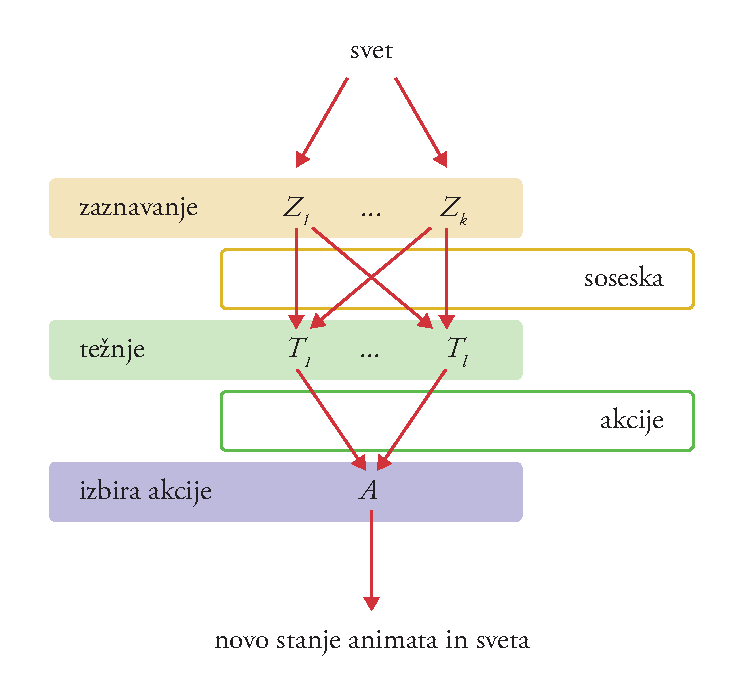
\includegraphics[width=.6\figurewidth]{fig_animat_si}
	\vskip.2in
	\caption{Vizualizacija procesov in terminologije povezanih z animatom.}
	\label{fig:animat_si}
\end{figure}

Animat torej povzema osnovne lastnosti pravih živali \cite{lebarbajec2005fuzzy}. Prav tako kot prave živali obstaja v prostoru in času, obkrožajo pa ga živi in neživi objekti, kar pomeni, da animat prebiva v nekem prostoru Animat se zaveda svojega trenutnega stanja in je sposoben zaznavanja stanja bližnje okolice. Ima težnje, ki jih preko izvajanja akcij poskuša zadovoljiti. Tako lahko preko akcij vpliva na svoje stanje ter na stanje prostora.

S pomočjo modelov, zasnovanih na nivoju posameznika, je bilo pokazano, da lahko do zapletenih dinamik skupinskega vedenja pridemo že, če posamezniki sledijo dokaj preprostim težnjam. Prvi poskusi modeliranja skupinskega vedenja s pomočjo modelov zasnovanih na nivoju posameznika segajo v osemdeseta leta prejšnjega stoletja. Aoki \cite{aoki1982simulation} je predlagal pristop od spodaj navzgor za simuliranje jat rib. Reynolds \cite{reynolds1987flocks} je razvil prvi računalniški model za proceduralno animiranje jat ptic. Podobno kot Reynolds sta tudi Heppner in Grenander \cite{heppner1990stochastic} modelirala jate ptic, a s pomočjo stohastičnih nelinearnih diferencialnih enačb. Poleg naštetih modelov se tudi večina novejših \cite{couzin2002collective,demsar2013family,demsar2014simulated,demsar2015simulating,demsar2016balanced,demsar2017evolution,helbing1995social,hildenbrandt2010selforganized,lebarbajec2009organized,parrish2002schools,schellinck2011review,sumpter2006principles,vicsek2012collective} razlikuje zgolj v implementaciji določenega segmenta animata, glavni del, ki definira vedenje, pa je v večini modelov zelo podoben. Vedenje animatov v večini primerov temelji na treh težnjah (Slika~\ref{fig:drives_si}), ki se imenujejo razmik (\angl{separation}), poravnava (\angl{alignment}) in kohezija (\angl{cohesion}). S kohezijo modeliramo težnjo biti blizu drug drugemu. Tako se animat, če nima bližnjih sosedov, želi približati tistim, ki so bolj oddaljeni. S pomočjo težnje razmika animati ohranjajo osebni prostor ter preprečujejo trke. S pomočjo poravnave usklajujejo smer in hitrost gibanja s sosedi. Ker se lahko že zgolj s poravnavo smeri gibanja prepreči razpadanje skupin ter medsebojne trke, nekateri modeli uporabljajo izključno to težnjo \cite{vicsek1995novel}.

\begin{figure*}
	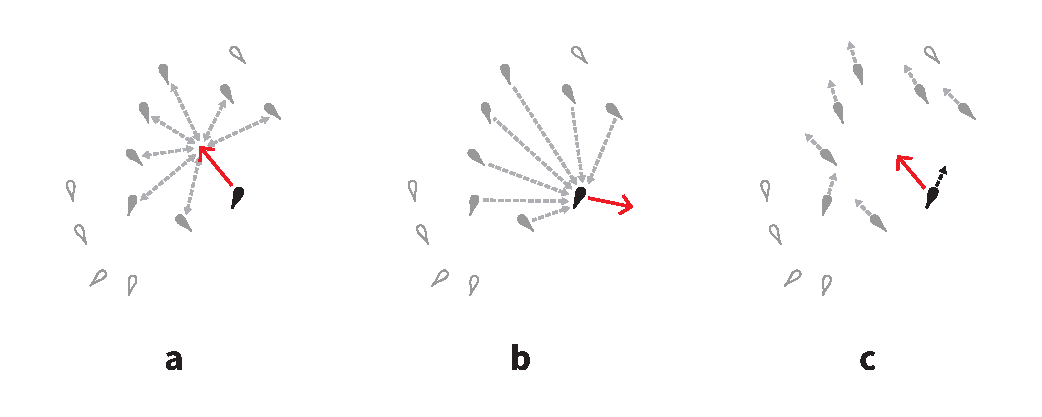
\includegraphics[width=\figurewidth]{figDrives}
	\caption{Vizualizacije treh osnovnih teženj: (a) kohezija, (b) razmik in (c) poravnava. Črni animat je opazovani posameznik. Sivi animati so sosedi, ki neposredno vplivajo na vedenje opazovanega posameznika. Beli animati s sivo obrobo so sosedi, ki nimajo neposrednega vpliva na vedenje opazovanega posameznika.}
	\label{fig:drives_si}
\end{figure*}

%-----
\section{Evolucijski animat}

Nekoliko drugačen pristop predstavljajo modeli, kjer vedenje animatov ni načrtovano povsem ročno, ampak lahko animati svoje vedenje skozi čas spreminjajo samodejno (pri ročno načrtovanih modelih se obnašanje animatov skozi čas ne spreminja). Spremembe vedenja izvajajo za dosego čimbolj učinkovitega zadovoljevanja teženj v danem okolju oziroma prostoru. Običajno so taki modeli osnovani na genetskih algoritmih, ki s pomočjo selekcije, križanja in mutacije posnemajo naravno evolucijo in tako iščejo rešitve za razne kompleksne probleme \cite{goldberg1989genetic,goldberg2002design,holland1992adaptation}. Selekcija zagotavlja, da imajo boljše rešitve oziroma boljši osebki večjo možnost za reprodukcijo. S tem se zagotovi prenos dobrega genetskega materiala v naslednje generacije. Kvaliteta posamezne rešitve se ocenjuje s pomočjo ocenjevalne funkcije. Križanje posnema izmenjavo genetskega materiala pri reprodukciji. Pri formiranju novega osebka se tako kromosomi staršev združijo v en kromosom, ki opredeljuje otroka. S tem se lastnosti staršev prenesejo na otroke. V naravi razne anomalije v reprodukcijskem procesu povzročijo spremembe v genetskem materialu, kar vodi v mutacije, zato genetski algoritmi v zadnjem koraku opravljajo še mutacije -- redke naključne spremembe otrokovega kromosoma. 

Pri najbolj pogosti uporabi genetskih algoritmov so generacije osebkov med seboj običajno povsem ločene. Pred generiranjem nove generacije se najprej oceni kvaliteta vseh rešitev v trenutni generaciji, nato pa se preko izvajanja operacij selekcije, križanja in mutacije ustvari nova enako velika generacija.

V zadnjem času je bilo obljavljenih več pomembnih člankov \cite{kunz2006prey,olson2013predator,olson2016evolution,biswas2014causes,demsar2015simulating,demsar2016balanced,demsar2017evolution,hein2015evolution}, ki so uporabili genetske algoritme za analizo različnih hipotez o evoluciji skupinskega vedenja. Nekateri izmed teh \cite{sayers2009evolved,spector2003emergence,wood2007evolving} so genetske algoritme uporabili predvsem za prilagajanje parametrov v diferencialnih enačbah, ki definirajo znane težnje (težnje izhajajoče iz ne-evolucijskih modelov). Glavna težava pristopa je, da uporaba znanih teženj verjetno usmerja tok evolucije proti razvoju znanega (skupinskega vedenja). Reynolds je bil prvi, ki je uporabil kombinacijo genetskih algoritmov in genetskega programiranja \cite{koza1992genetic} za simuliranje evolucije skupinskega vedenja, ne da bi uporabil vnaprej definirane težnje \cite{reynolds1993evolved}. Vedenje, ki se je v njegovem primeru razvilo, težko primerjamo s kompleksnimi pojavi skupinskega vedenja v naravi. Glavni razlog verjetno tiči v tem, da je bil Reynoldsov model pretirano poenostavljen. Zaera in sod. so pri poskusu simuliranja evolucije skupinskega vedenja uporabili kombinacijo umetnih nevronskih mrež in genetskih algoritmov. Njihov poskus se ni končal najbolje, saj jim ni uspelo razviti vedenja, ki bi bilo podobno primerom iz narave. Po prepričanju avtorjev je glavni razlog za spodletel poskus v ocenjevalni funkciji. Ugotovili so, da je težko definirati ocenjevalno funkcijo, ki dobro opiše pojav skupinskega vedenja s stališča posameznika. Ocenjevalna funkcija je ključni element pri genetskih algoritmih, saj določa, katere rešitve bodo v procesu evolucije vplivale na prihodnje rodove, katere pa bodo izumrle.

Ocenjevanje skupinskega vedenja s stališča posameznika je problematično vsaj z dveh stališč. Definicija stopnje oziroma kvalitete skupinskega vedenja ni najbolj jasna, tako s stališča posameznika kot skupine. V naravi namreč obstaja mnogo različnih režimov skupinskega vedenja. Vsak izmed njih je čudovit in spektakularen na svoj način. Neposredno ocenjevanje stopnje skupinskega vedenja obenem eksplicitno usmerja evolucijo proti razvoju skupinskega vedenja -- posameznike sili k izvajanju akcij, ki povečajo stopnjo skupinskega vedenja. Pri tradicionalni rabi genetskih algoritmov (ko gre za iskanje čim bolj optimalnih rešitev pri kompleksnih nalogah) takšno usmerjanje sicer ni problematično, se pa izkaže kot problematično, ko želimo uporabiti genetske algoritme za raziskovanje možnih vzrokov za razvoj skupinskega vedenja. Pri tovrstnih raziskavah nas bolj kot optimalna znana rešitev zanima, če se bo med animati skupinsko vedenje razvilo samodejno (brez eksplicitnega siljenja s strani ocenjevalne funkcije), kot odgovor na razne zunanje pritiske, ki so prisotni med simulirano evolucijo. 

Vrsta novejših raziskav \cite{biswas2014causes,hein2015evolution,olson2013predator,olson2015exploring,olson2016evolution,witkowski2016emergence} je pokazala, da se skupinsko vedenje razvije tudi z uporabo bolj prikrite ocenjevalne funkcije, in sicer takšne, ki ne usmerja evolucije k razvoju skupinskega vedenja eksplicitno. V omenjenih raziskavah je bila ocenjevalna funkcija zasnovana na sposobnosti preživetja v raznih neugodnih umetnih okoljih. Za preživetje v teh okoljih so animati morali izvajati akcije podobne tistim, ki jih izvajajo živali v naravi -- izmikanje plenilcem, iskanje hrane, itd. Animati, ki so bili pri tem bolj uspešni, so imeli več priložnosti za reprodukcijo. Na ta način so se skozi evolucijo ohranjali zgolj tisti animati, ki so izvajali akcije, s katerimi so uspeli čim več časa preživeti v danem neugodnem okolju. Skupinska vedenja, ki so se v omenjenih raziskavah razvila \cite{biswas2014causes,hein2015evolution,olson2013predator,olson2015exploring,olson2016evolution,witkowski2016emergence}, lahko uvrstimo v dva režima vedenja -- gručenje (\angl{clumping}) in rojenje (\angl{swarming}). V nobeni izmed omenjenih študij se niso razvile usklajene oblike gibanja, ki jih v naravi lahko občudujemo pri jatah rib in ptic -- kroženje okrog praznega jedra (\angl{milling}) oziroma dinamično usklajeno gibanje (\angl{dynamic parallel movement}) \cite{couzin2002collective,sumpter2006principles}.

%-----
\section{Mehki animat}

Najbolj pogosta pristopa za implementacijo animatov sta uporaba diferencialnih enačb \cite{couzin2002collective,hildenbrandt2010selforganized,reynolds1987flocks,vicsek2012collective} ali umetnih nevronskih mrež \cite{kunz2006prey,witkowski2016emergence,zaera1996not}. Umetne nevronske mreže so univerzalni funkcijski aproksimator, ki deluje po vzoru človeških oziroma živalskih možganov. Pristopa sta bila osnova številnih raziskav, ki so pripomogle k večjemu poznavanju skupinskega vedenja. Toda vsak izmed njiju ima določene pomanjkljivosti, ki zavirajo morebiten nadaljnji napredek. Pri diferencialnih enačbah je potrebno podrobno poznavanje vrednosti vseh parametrov modela, za prilagajanje in nadgrajevanje pa potrebujemo dobro matematično znanje. Glavna hiba pristopov, ki uporabljajo umetne nevronske mreže, je težavnost izluščevanja logike delovanja. Hiba je splošno znana in nekateri raziskovalci umetne nevronske mreže posledično označujejo kot pristop s »črno škatlo« \cite{paruelo1997prediction,lek1999artificial,ozesmi1999artificial}.

Lebar Bajec in sod. \cite{lebarbajec2005fuzzy,lebarbajec2005simulating} so za reševanje nekaterih od naštetih težav predlagali uporabo mehke logike (\angl{fuzzy logic}) \cite{zadeh1965fuzzy}. Mehka logika je univerzalni funkcijski aproksimator, tako kot umetne nevronske mreže. Ena izmed glavnih prednosti mehke logike je njena moč, ko operiramo s parametri modela, ki niso povsem natančno znani (so pomanjkljivi, dvoumni, oziroma dvomni). Druga prednost mehke logike je ta, da pri modeliranju uporablja lingvistične opise (če-potem pravila), ki so zelo podobni stavkom, ki jih ljudje tvorimo pri vsakodnevni komunikaciji \cite{kosko1994fuzzy,lebarbajec2005fuzzy,lebarbajec2005simulating,mamdani1975experiment,mendel2001uncertain,zadeh1965fuzzy}. Uporabnost mehke logike za razmeroma preprost prenos opažanj iz narave v modele ter učinkovito modeliranje naravnih pojavov so potrdile že številne raziskave \cite{dasilva2008predator,demsar2013family,demsar2014simulated,demsar2016balanced,demsar2017evolution,lebarbajec2005fuzzy,lebarbajec2005simulating,tron2004mathematical}.

Leta 2005 so Lebar Bajec in sod. predstavili definicijo mehkega animata (\angl{fuzzy animat}) \cite{lebarbajec2005fuzzy,lebarbajec2005simulating}, umetnega živega bitja, zasnovanega s pomočjo mehke logike. Glavna razlika med klasičnim animatom in mehkim animatom je v definiciji pristopa k implementaciji teženj. V primeru klasičnega animata so težnje običajno zapisane v obliki diferencialnih enačb, pri mehkih animatih pa so težnje zapisane v obliki mehkega odločitvenega sistema (\angl{fuzzy rule-based system}). Mehki odločitveni sistem je opredeljen z mehko bazo znanja (\angl{fuzzy knowledge base}), ki je sestavljena iz mehke baze podatkov (\angl{fuzzy data base}) in mehke baze pravil (\angl{fuzzy rule base}). V prvi so deklarirane mehke spremenljivke, mehke vrednosti in interpretacija logičnih povezav. Mehka baza pravil podaja opis obnašanja sistema. V ta namen uporablja lingvistični opis, če-potem pravila v katerih nastopajo logične povezave, mehke spremenljivke in vrednosti. Primer enostavne mehke baze znanja pri sistemu za gretje prostora je predstavljen na sliki~\ref{fig:knowledgebase_si}.

\begin{figure}
	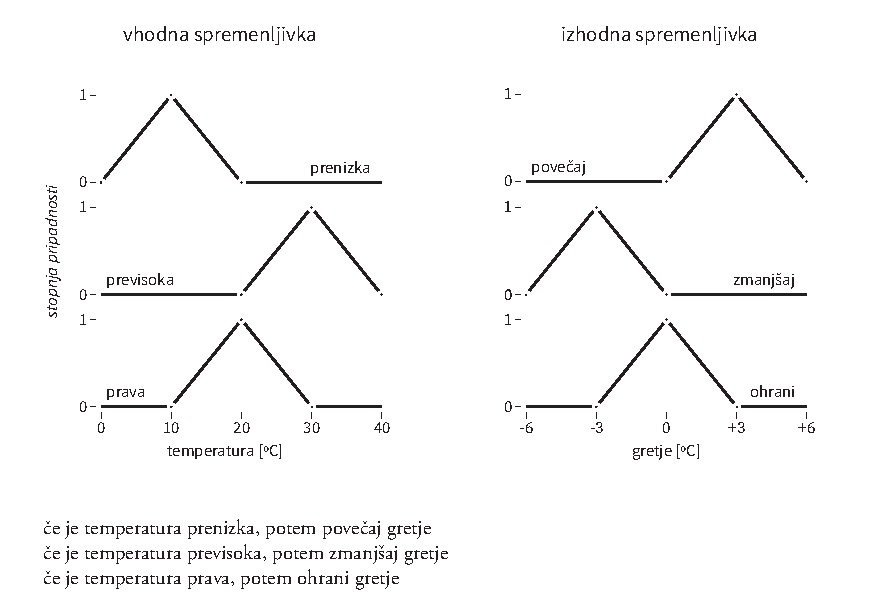
\includegraphics[width=\figurewidth]{figKnowledgebase_si}
	\caption{Primer enostavne mehke baze znanja. Primer prikazuje mehki sistem za gretje prostora. Zgornji del vizualizira mehko bazo podatkov, definirani imamo dve mehki spremenljivki -- eno vhodno in eno izhodno. Vhodna spremenljivka je trenutna temperatura v prostoru, ki jo sistem pridobi s pomočjo senzorja za temperaturo. Mehka baza pravil (spodnji del) opisuje, kako se vhodne spremenljivke pretvorijo v akcije (izhodne spremenljivke) preko če-potem pravil. V našem primeru je akcija sistema za gretje sprememba v temperaturi prostora.}
	\label{fig:knowledgebase_si}
\end{figure}

V primeru animatov mehka baza podatkov definira, kako animati interpretirajo svojo okolico oziroma informacije, ki jih dobijo iz okolice s pomočjo zaznavanja (na primer razdaljo do najbližjega soseda, smer gibanja plenilca, položaj ovire, itd.) ter definira akcije, ki jih lahko izvajajo za spremembo lastnega stanja in/ali stanja prostora (na primer spremembo hitrosti, spremembo smeri gibanjam itd.). Kako mehki animat pretvori pridobljene informacije v akcije je definirano v mehki bazi pravil.

%-----
\section{Cilj: evolucijski mehki animat}

Glavni cilj pričujoče disertacije je bil razvoj umetnega genetskega sistema, primernega za simuliranje evolucije pojavov skupinskega vedenja s pomočjo mehke logike. Ker najbolj pogosta hipoteza o nastankih skupinskega vedenja trdi, da se je pojav morda razvil kot zaščita pred plenilci \cite{cresswell2011predicting,hart2005predator,krause2002living,larsson2012why,lebarbajec2009organized,nishimura2002predator,pavlov2000patterns}, lahko predpostavimo, da je boj za preživetje med plenilci in plenom verjetno smiseln del evolucijskega modela. Da bi pri konstrukciji in validaciji evolucijskega modela naleteli na čim manj težav, smo se odločili, da bomo najprej preučili dinamiko med plenilci in plenom v ročno načrtovanem modelu. S pomočjo analize taktik napada v ročno načrtovanem modelu \cite{demsar2014simulated} smo pridobili tako znanje o taktikah napada, ki jih uporabljajo plenilci, kot tudi vpogled v reakcije plena ob napadu plenilca. Med študijo smo spoznali, da plenilci v računalniških modelih večinoma uporabljajo zgolj osnovne taktike napada. Po drugi strani pa plenilci, ki v naravi napadajo plen, ki se zadržuje v skupinah, uporabljajo različne in pogostokrat zelo izdelane taktike napada. Zato smo v naslednjem koraku razvili evolucijski model, v katerem plenilci prilagajajo taktike napada s ciljem doseganja čim višje uspešnosti pri lovu. Z raziskavo smo skušali dobiti odgovor na vprašanje o optimalni taktiki napada v odvisnosti od režima skupinskega vedenja oziroma odziva plena \cite{demsar2015simulating}.

S pomočjo znanja, pridobljenega v okviru teh dveh raziskav, smo nato razvili umetni genetski mehki sistem (\angl{genetic fuzzy system}), ki je primeren za simuliranje evolucije skupinskega vedenja. Genetski mehki sistemi \cite{cordon2001genetic,cordon2004ten,fernandez2015revisiting,herrera1996genetic,herrera2008genetic,pedrycz1996fuzzy,sanchez1997genetic} izkoriščajo genetske algoritme za optimizacijo ali konstrukcijo mehkih baz znanja. Večina genetskih mehkih sistemov se ukvarja z optimizacijo ročno načrtovanih mehkih sistemov \cite{cordon2004ten,fernandez2015revisiting,herrera2008genetic}. Zahtevnejši pristop je genetsko učenje mehkih sistemov (\angl{genetic learning of fuzzy systems}), pri katerem se genetski algoritmi ne uporabljajo zgolj za optimizacijo obstoječih mehkih sistemov, ampak se komponente sistema (mehko bazo znanja, mehko bazo podatkov, ali mehko bazo pravil) ustvari kar s pomočjo genetskih algoritmov. V tej disertaciji se osredotočamo na ustvarjanje mehkih baz pravil (tudi genetsko učenje pravil) animatov. Pri animatih je mehka baza pravil verjetno najbolj pomemben del mehkega sistema, saj je v njej zapisano kako animat zaznane informacije pretvori v akcije.

V literaturi lahko najdemo dva prevladujoča pristopa k genetskemu učenju pravil -- michiganski pristop \cite{holland1977cognitive} in pittsburški \cite{smith1980learning} pristop. Pri prvem kromosom v genetskem algoritmu predstavlja posamezno pravilo, kar pomeni, da celotna generacija predstavlja eno samo mehko bazo pravil. Kvaliteta (ocena) mehke baze pravil (ustreznost za reševanje danega problema) torej narašča skozi povsem ločene generacije. V našem primeru bi to pomenilo, da je vsem animatom dodeljena identična baza pravil. Ker tega nismo želeli, smo se odločili za uporabo pittsburškega pristopa. Pri tem posamezen kromosom predstavlja celotno mehko bazo pravil. Na tak način smo lahko vsak animat obravnavali kot posameznika (vsak animat je definiran s svojim kromosomom). S tem smo se tudi odmaknili od klasične uporabe genetskih algoritmov, kjer so generacije med seboj povsem ločene in se približali simuliranju umetnega življenja (\angl{artificial life}), kjer ni povsem jasnih medgeneracijskih mej -- selekcija, križanje in mutacija so del odvijajoče se evolucije. Ker je v našem sistemu vsak animat definiran s svojim kromosomom, je rezultat heterogena populacija animatov (heterogena po obnašanju in ne po fiziologiji). Tako bi lahko rekli, da se animati, preko svojih mehkih baz pravil, borijo za preživetje v okolju, ki je tekmovalno iz dveh pogledov. Prvi del boja za preživetje animati bijejo s plenilci, drugi del pa med seboj, ko si poskušajo izboriti večjo možnost za reprodukcijo. S tem pristopom ter z uporabo različnih taktik napada pri plenilcih nam je uspelo razviti mehki genetski sistem, ki je sposoben generirati večji nabor režimov skupinskega vedenja \cite{demsar2017evolution}, kot so jih sposobne reproducirati obstoječe raziskave \cite{biswas2014causes,hein2015evolution,olson2013predator,olson2015exploring,olson2016evolution,reynolds1993evolved,sayers2009evolved,spector2003emergence,wood2007evolving}. Sistem smo nato v nadaljevanju uporabili za analizo vpliva različnih sočasnih pritiskov na obliko skupinskega vedenja, ki nastane ob evoluciji \cite{demsar2016balanced}.

%-----
\section{Rezultati}

V prvi fazi raziskav smo razvili nov mehki model \cite{demsar2014simulated} za simulacijo letenja ptic v jati, ko so te izpostavljene napadom plenilca. Interakcija v modelu in taktike napada temeljijo na vizualni zaznavi. Pri tem upoštevajo prekrivanje oddaljenih predmetov s strani bližnjih \cite{kunz2012simulations} in omejitve delovnega spomina \cite{ballerini2008interaction,engle1999individual,sherry1989hippocampus}. Taktike napada plenilca so bile tri -- napad najbližjega izmed vidnih animatov, napad najbolj vizualno ločenega izmed vidnih animatov in sredine skupine vidnih animatov. V raziskavi smo obravnavali dva režima vedenja plena, in sicer socialno, kjer se animati z upoštevanjem nagonov kohezije in poravnave aktivno združujejo v jate in individualno, kjer tega ne počnejo (izogibajo se zgolj trkom). Rezultati kažejo, da je najbolj uspešen plenilec tisti, ki lovi vizualno ločene osebke, a to predvsem v primerih, ko je vedenje plena socialno. Ko je vedenje plena individualno, je s stališča plenilca najboljša taktika napad najbližjega. S stališča plena je socialno vedenje boljše, saj ne glede na taktiko napada plenilca podaljša čas, ki ga slednji potrebuje za ulov. To krepi hipotezo, da se je združevanje v skupine lahko razvilo kot zaščita pred plenilci. Obenem pa nakazuje, da je najboljša taktika plenilca močno odvisna od vedenja plena.

V drugi fazi smo nato razvili evolucijski model \cite{demsar2015simulating}, v katerem smo s pomočjo genetskih algoritmov prilagajali parametre, s katerimi so bile definirane ročno načrtovane taktike napada. S pomočjo prilagajanja parametrov taktik se je plenilcem skozi čas povečala uspešnost pri lovu. Z namenom lažje primerljivosti z ostalimi raziskavami smo se osredotočili na znane osnovne taktike napada (napad najbližjega, napad najbolj izoliranega in napad najbolj središčnega animata, ki predstavlja plen), a tem dodali še napredno dvofazno taktiko. S to taktiko, ki smo jo poimenovali razpršilna (\angl{dispersing}), se plenilec najprej usmeri v središče jate, da bi v njej povzročil kaos in njen razkroj, nato pa se osredotoči na najbolj izolirane posameznike. Taktiko uporablja več vrst plenilcev v naravi \cite{larsson2012why,pavlov2000patterns}. V raziskavi smo nato obravnavali tako vpliv zmedljivosti plenilca, kot tudi kaj se zgodi, če plen, ki se združuje v jate, kot obrambni mehanizem izvaja manever zakasnjenega odziva, kjer se na napad ne odzove ob prvi zaznavi plenilca, ampak odziv zakasni. Rezultati kažejo, da je razpršilna taktika najuspešnejša in edina sposobna vsaj v določeni meri izničiti uspešnost zakasnjenega odziva kot obrambne taktike plena. Ker je uspešnost plenilca s prilagajanjem razpršilne taktike bistveno upadla, če ta ni bil zmedljiv, slednje nakazuje, da je zmedljivost lahko igrala pomembno vlogo v evoluciji naprednih taktik napada.

Glede na znanje pridobljeno s predhodnimi fazami raziskave smo z namenom evolucije skupinskega vedenja v tretji fazi razvili genetski mehki sistem \cite{demsar2017evolution}, ki temelji na umetnem življenju. Animati, ki predstavljajo plen, so se razvijali pod sočasnimi pritiski plenilcev, ki uporabljajo več ročno načrtovanih taktik napada (napad najbližjega posameznika, napad najbolj izoliranega posameznika, napad najbolj središčnega posameznika in napad najgostejšega predela skupine). S prvimi tremi taktikami plenilec lovi in ujame zgolj enega samega posameznika, pri zadnji pa plenilec lahko lovi in ujame več posameznikov hkrati (kot to v naravi počno nekatere vrste morskih kitov \cite{domenici2001scaling,goldbogen2011mechanics,nottestad1999herring,nottestad2002whales}). Ker so animati, ki predstavljajo plen, sobivali v okolju s plenilci, pri čemer je bil cilj prvih preživeti, drugih pa ujeti čim več posameznikov, je nastanek skupinskega vedenja pogojen zgolj s tem, da animatom v tem okolju pomaga preživeti čim dlje. Rezultati kažejo, da model razvije večje število režimov skupinskega vedenja, kot obstoječe raziskave \cite{biswas2014causes,hein2015evolution,olson2013predator,olson2015exploring,olson2016evolution,reynolds1993evolved,sayers2009evolved,spector2003emergence,wood2007evolving}. Analiza mehkih pravil je pokazala, da se režimi vedenja statistično značilno razlikujejo po deležu pravil, ki upoštevajo plenilca.

V četrti fazi raziskav smo zato izvedli kontroliran eksperiment evolucije, kjer smo sistematično izbirali taktike napada, katerim so bili animati med evolucijo izpostavljeni \cite{demsar2016balanced}. Osredotočili smo se na to, kako različni pritiski vplivajo na režim skupinskega vedenja, ki se razvije. Rezultati potrjujejo dotedanje raziskave \cite{biswas2014causes,olson2013predator,olson2016evolution,wood2007evolving}, da se a) v primeru taktik napada na najbližjega oz. najbolj izoliranega posameznika razvije združevanje v skupine, ter da se b) v primeru taktik napada na najbolj središčnega posameznika oz. najgostejši del jate razvije razprševanje. V teh primerih so se razvile oblike gibanja, ki so najbolj podobne rojenju oziroma kroženju okrog praznega jedra. Najbolj zanimivi rezultati so nastali v primerih, ko so bili animati izpostavljeni taktikam, od katerih nekatere usmerjajo evolucijo plena k združevanju v skupine, nekatere pa k razpršitvi. Zgolj v teh primerih so se namreč razvile usklajene oblike gibanja, ki jih v naravi občudujemo v jatah ptic in rib (dinamično usklajeno gibanje in močno usklajeno gibanje).

Vsaka izmed faz predstavlja lasten izviren doprinos k znanosti in vsaka je bila predstavljena v svojem izvirnem znanstvenem prispevku \cite{demsar2014simulated,demsar2015simulating,demsar2017evolution,demsar2016balanced}.

%-----
\section{Nadaljne raziskave}

V procesu raziskav, predstavljenih v pričujoči disertaciji, se nam je porodilo več idej, ki bi lahko bile potencialno zanimive za nadaljnje raziskave skupinskega vedenja. Pri uporabi evolucijskih modelov za iskanje odgovora na biološka vprašanja so verjetno trenutno največja hiba poenostavitve modelov, ki se jih raziskovalci poslužujejo zaradi velike računske zahtevnosti tako genetskih algoritmov, kot že samih računalniških modelov skupinskega vedenja. Za zvišanje biološke relevantnosti evolucijskih modelov bi bilo dobro odstraniti čim več poenostavitev. Med najbolj pogoste sodijo omejitev gibanja animatov na dve dimenziji, nerealistični sistemi zaznavanja, gibanje s konstanto hitrostjo, itd. Če na primer hočemo animatom v evolucijskih modelih omogočiti spreminjanje hitrosti, bo verjetno potrebno najprej implementirati porabo energije, ki bo posledično vodila v to, da se animati lahko tudi utrudijo. S tem se animati, prav tako kot živa bitja v naravi \cite{norin2016measurement,roche2013finding}, ne bi mogli ves čas premikati z maksimalno hitrostjo, ki jo lahko dosežejo. 

Ena izmed možnih smeri nadaljnih raziskav bi lahko bila tudi analiza vpliva heterogenosti v fiziologiji na evolucijo skupinskega vedenja. Nekatere aktualne raziskave namigujejo, da heterogene skupine v evolucijskem modelu razvijejo drugačno vedenje, kot homogene \cite{olson2015exploring}. Druge nakazujejo, da je heterogenost morda pomembna za dosego bolj ``naravnega'' vedenja \cite{demsar2013family} in da so morda razlike med posamezniki pomembne za koordinacijo skupine \cite{marras2012information,marras2013schooling}. V naravi je heterogenost (tako v vedenju kot v fiziologiji) vedno prisotna. Na primer ptice se v jatah pogosto razlikujejo v velikosti, spolu, starosti in včasih celo v vrsti \cite{lebarbajec2009organized,jolles2013heterogeneous}. Tako pogosto vidimo, da se močnejši posamezniki nahajajo v najbolj varnih predelih skupine \cite{hamilton1971geometry}, posledično pa so šibkejši posamezniki bolj izpostavljeni napadom plenilcev. Nekateri plenilci v naravi celo namenoma napadajo šibkejše posameznike \cite{domenici2014howsailfish,marras2015notsofast}. Z razvojem modela, v katerem bi bili animati heterogeni tudi po fiziologiji, bi lahko, poleg vpliva heterogenosti na evolucijo skupinskega vedenja, analizirali tudi to, kako plenilci prilagodijo svoje taktike napada pri napadu heterogenih skupin.

V večini obstoječih modelov \cite{demsar2014simulated,demsar2015simulating,demsar2016balanced,demsar2017evolution,nishimura2002predator,zheng2005behavior} plenilec za sledenje izbrani tarči uporablja tehniko klasičnega zasledovanja (\angl{classical pursuit}) \cite{nahin2012chases}. V naravi najdemo tudi plenilce, ki uporabljajo bolj napredne tehnike sledenja tarči. Nekatere vrste sokolov uporabljajo tehnike sledenja, s katerimi zakrivajo svojo smer gibanja (\angl{motion camouflage}) \cite{kane2014falcons}. To dosežejo na več načinov. Tarčo lahko pretentajo s pomočjo objektov v ozadju, ali pa se ji približujejo pod takim kotom, da tarča tega približevanja ne opazi \cite{justh2006steering}. Tako bi lahko s pomočjo genetskih algoritmov poleg taktik napada razvijali tudi taktike sledenja, ali pa bi celo sočasno razvijali skupinsko vedenje in taktike sledenja plenilcev. Na njihovo soodvisnost so opozorile že naše uvodne raziskave.

V naravi pogosto lahko opazimo tudi pojav skupinskega lova \cite{creel1995communal,escobedo2014groupsize,fanshawe1993factors,lett2004continuous,muro2011wolfpack,packer1988evolution,scheel1991group}. Pri skupinskem lovu več plenilcev sodeluje med sabo in si s tem izboljša možnosti za uspešen ulov. Čeprav je v naših modelih lahko sočasno aktivnih več plenilcev, le-ti ne sodelujejo med sabo. Analiza evolucije sodelovanja plenilcev med lovom bi verjetno privedla do zanimive raziskave in rezultatov.

Nenazadnje, eno izmed pomembnih vprašanj je, kdaj se bo plen po zaznavi napada odločil začeti bežati. V naravi nekatere vrste rib kot obrambni mehanizem namensko zakasnijo odziv \cite{partridge1982structure}. Naše raziskave so že nakazale, da je omenjeni manever pri določenih taktikah napada uspešen. Evolucijski model pa omogoča pridobiti odgovore na vprašanje pod kakšnimi pogoji se tak zakasnjen odziv razvije. Raziskave v tej smeri že izvajamo in trenutni rezultati nakazujejo, da se odgovor morda navezuje na razmerja v hitrostih med plenilcem in plenom.

S pomočjo evolucijskih modelov smo razvozlali že marsikatero uganko glede skupinskega vedenja, glede na trenutne smernice pa verjamemo, da najzanimivejši odgovori šele prihajajo.

\end{razsirjeniPovzetek}

\end{document}
